\documentclass[tikz,border=2pt]{standalone}
\usepackage{tikz}

\begin{document}
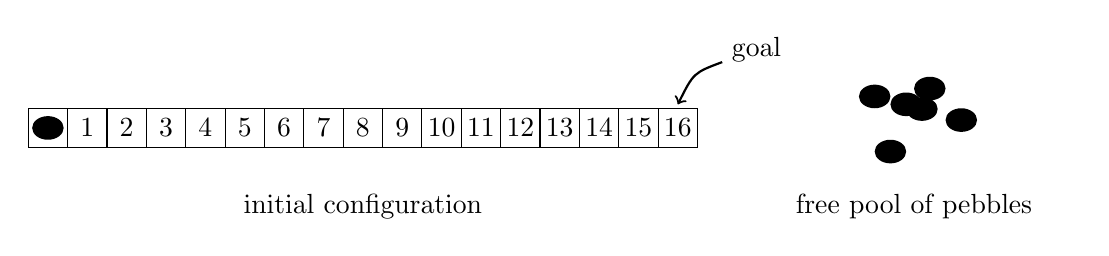
\begin{tikzpicture}[scale=1.0]

\def\y{0}
\node at (4, \y-1) {initial configuration};
\foreach \x in {0,...,16}{
	\draw (0.5*\x-0.25, 0.5*\y-0.25) rectangle (0.5*\x+0.25, 0.5*\y+0.25);
	\ifnum \x > 0
		\node at (0.5*\x, 0.5*\y) {\x};
	\fi
}
\fill (0, 0)  ellipse (0.2 and 0.15);
\def\dx{11}
\foreach \a/\b in {-0.1/0.3, 0.2/0.5, -0.5/0.4, 0.1/0.24, 0.6/0.1, -0.3/-0.3}
	\fill (\dx+\a, \y+\b)  ellipse (0.2 and 0.15);
\node at (11, -1) {free pool of pebbles};
\node at (13, -1) {};
\node (goal) at (9, \y+1) {goal};
\draw[<-,thick] (8, \y+0.3) .. controls (8.2, \y+0.7) .. (goal);

\end{tikzpicture}
\end{document}
